\documentclass{standalone}
\makeatletter\AtBeginDocument{\@buildstepset{1,2,3,4}}\makeatother
\usepackage{tikz}
\usetikzlibrary{intersections, calc}
\usepackage{hsbcommon}
\begin{document}
    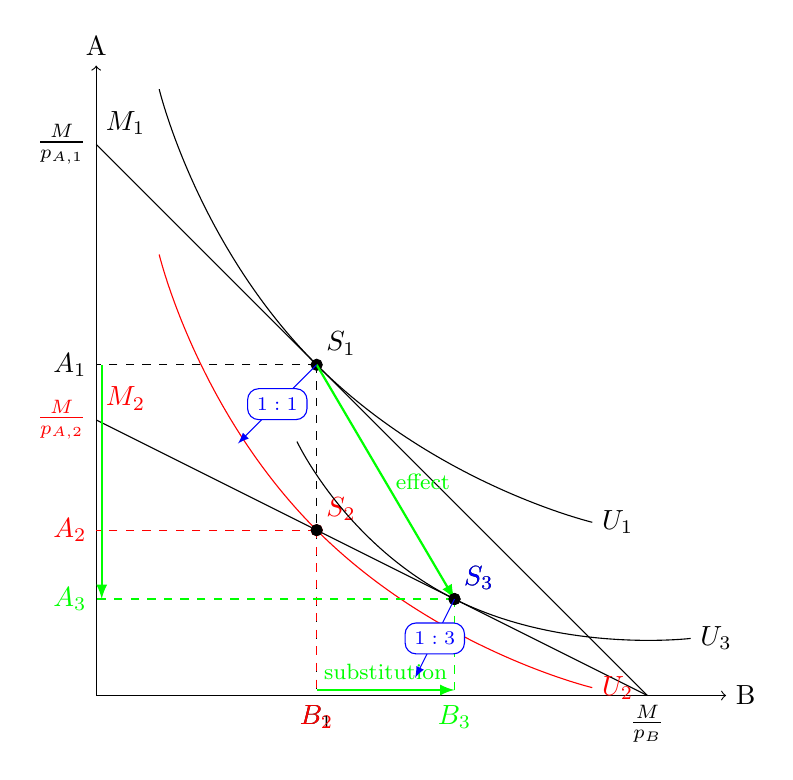
\begin{tikzpicture}
        \draw[->] (0,0) node[below] {\phantom{$X_i$}} -- (8,0) node[right]  {B};
        \draw[->] (0,0) node[left] {\phantom{$Y_mi$}} -- (0,8) node[above]  {A};

        %% Always visible: first budget line (black) + indifference curve U_1
        \begin{scope}[color=black]
            \coordinate (A1) at (0,7);
            \coordinate (B1) at (7,0);
            \node[above right] at (A1) {$M_1$};
            \node[left]        at (A1) {$\frac{M}{p_{A,1}}$};
            \node[below]       at (B1) {$\frac{M}{p_B}$};
            \draw [name path=budgetgerade1, opacity=1, color=black]
                plot [smooth] coordinates {(A1)(B1)};
            \coordinate (S1) at ($(A1)!0.4!(B1)$);
            \node[above right] at (S1) {$S_1$};
            \coordinate (s1) at (S1);
            \draw [dashed] (S1) -- (S1 |-,0) node [below] {$B_1$};
            \draw [dashed] (S1) -- (0,|- S1)  node [left]  {$A_1$};
            \filldraw (S1) circle (2pt);
            \coordinate (myP) at ([shift=({-2cm,3.5cm})]S1);  %% upper-left ctrl point
            \coordinate (myQ) at ([shift=({3.5cm,-2cm})]S1);  %% lower-right ctrl point
            \node[right] at (myQ) {$U_1$};
            \draw [name path=indiff1] plot [smooth, tension=1] coordinates {(myP)(S1)(myQ)};
        \end{scope}

        %% Step 1: second budget line (red, pivoted) + indifference curve U_2
        \ifstep{1}{
            \begin{scope}[color=red]
                \coordinate (A2) at (0,3.5);
                \coordinate (B2) at (7,0);
                \node[above right] at (A2) {$M_2$};
                \node[left]        at (A2) {$\frac{M}{p_{A,2}}$};
                \draw [name path=budgetgerade2, opacity=1, color=black]
                    plot [smooth] coordinates {(A2)(B2)};
                \coordinate (S2) at ($(A2)!0.4!(B2)$);
                \node[above right] at (S2) {$S_2$};
                \coordinate (s2) at (S2);
                \draw [dashed] (S2) -- (S2 |-,0) node [below] {$B_2$};
                \draw [dashed] (S2) -- (0,|- S2)  node [left]  {$A_2$};
                \filldraw (S2) circle (2pt);
                \coordinate (P2) at ([shift=({-2cm,3.5cm})]S2);
                \coordinate (Q2) at ([shift=({3.5cm,-2cm})]S2);
                \node[right] at (Q2) {$U_2$};
                \draw [name path=indiff2] plot [smooth, tension=1] coordinates {(P2)(S2)(Q2)};
            \end{scope}
        }

        %% Step 2: third point S_3 on new budget line + indifference curve U_3
        \ifstep{2}{
            \begin{scope}[color=black]
                \coordinate (s3) at ($(A2)!0.65!(B2)$);
                \filldraw (s3) circle (2pt);
                \node[above right] at (s3) {$S_3$};
                \coordinate (p3) at ([shift=({-2cm,2cm})]s3);
                \coordinate (q3) at ([shift=({3cm,-0.5cm})]s3);
                \node[right] at (q3) {$U_3$};
                \draw [name path=indiff3] plot [smooth, tension=1] coordinates {(p3)(s3)(q3)};
            \end{scope}
        }

        %% Step 3: erase old U_1, show substitution and income effects
        \ifstep{3}{
            \begin{scope}[color=green]

                \filldraw[black] (s2) circle (2pt);
                \draw[thick,->,>=latex] (s1) --
                    node[right] {\footnotesize effect} (s3);
                \draw [dashed] (s3) -- (s3 |-,0) node [below] {$B_3$};
                \draw [dashed] (s3) -- (0,|- s3)  node [left]  {$A_3$};
                \draw[thick,->,>=latex,xshift=2pt] (0,|- s1) -- (0,|- s3);

                \draw[thick,->,>=latex,yshift=2pt] (s2 |-,0) --
                    node[above] {\footnotesize substitution} (s3 |-,0);
            \end{scope}
        }

        %% Step 4: price-quantity ratios at S_1 and S_3
        \ifstep{4}{
            \begin{scope}[color=blue]
                \filldraw[black] (s3) circle (2pt);
                \node[above right] at (s3) {$S_3$};
                \draw[->,>=latex] (s3) --
                    node[fill=white,draw,rounded corners] {\scriptsize $1:3$}
                    ([shift=({-0.5cm,-1cm})]s3);
                \draw[->,>=latex] (s1) --
                    node[fill=white,draw,rounded corners] {\scriptsize $1:1$}
                    ([shift=({-1cm,-1cm})]s1);
            \end{scope}
        }

    \end{tikzpicture}
\end{document}
